% week-08 midterm: chaewoonee (26510127) Round 3 agent architecture, one page.
% Build: pdflatex architecture.tex   (or xelatex; no extra fonts needed)
\documentclass[10pt]{article}
\usepackage[a4paper,landscape,margin=8mm]{geometry}
\usepackage[T1]{fontenc}
\usepackage{helvet}
\renewcommand{\familydefault}{\sfdefault}
\usepackage{tikz}
\usetikzlibrary{positioning,fit,arrows.meta,calc,backgrounds}
\pagestyle{empty}
\definecolor{kit}{HTML}{ECECEC}
\definecolor{mine}{HTML}{DCEBFA}
\definecolor{ctx}{HTML}{FFF1D6}
\definecolor{model}{HTML}{E9DFF7}
\definecolor{mkt}{HTML}{E1F3E3}
\definecolor{loop}{HTML}{C0392B}
\definecolor{ink}{HTML}{1F2D3A}
% a red loop badge used inside box text: \lp{3}
\newcommand{\lp}[1]{\tikz[baseline=-0.6ex]\node[circle,draw=loop,fill=white,text=loop,font=\bfseries\scriptsize,inner sep=0.6pt,minimum size=3.2mm]{#1};}
\begin{document}
\color{ink}
\noindent{\Large\bfseries chaewoonee: Round 3 shop and buyer}\hfill{\small 26510127 \textbullet{} Week 08 midterm \textbullet{} kit v4 + my code}\\[2pt]
{\small\textbf{Design choice.} Code fixes every number that can lose money (cost floor, budget, target price, accept policy, forum text); the model only chooses inside those bounds. A context layer estimates what the market hides (what sells, what buyers want) from three clues: the public ledger, my own logs, and the forum.}

\vspace{2mm}
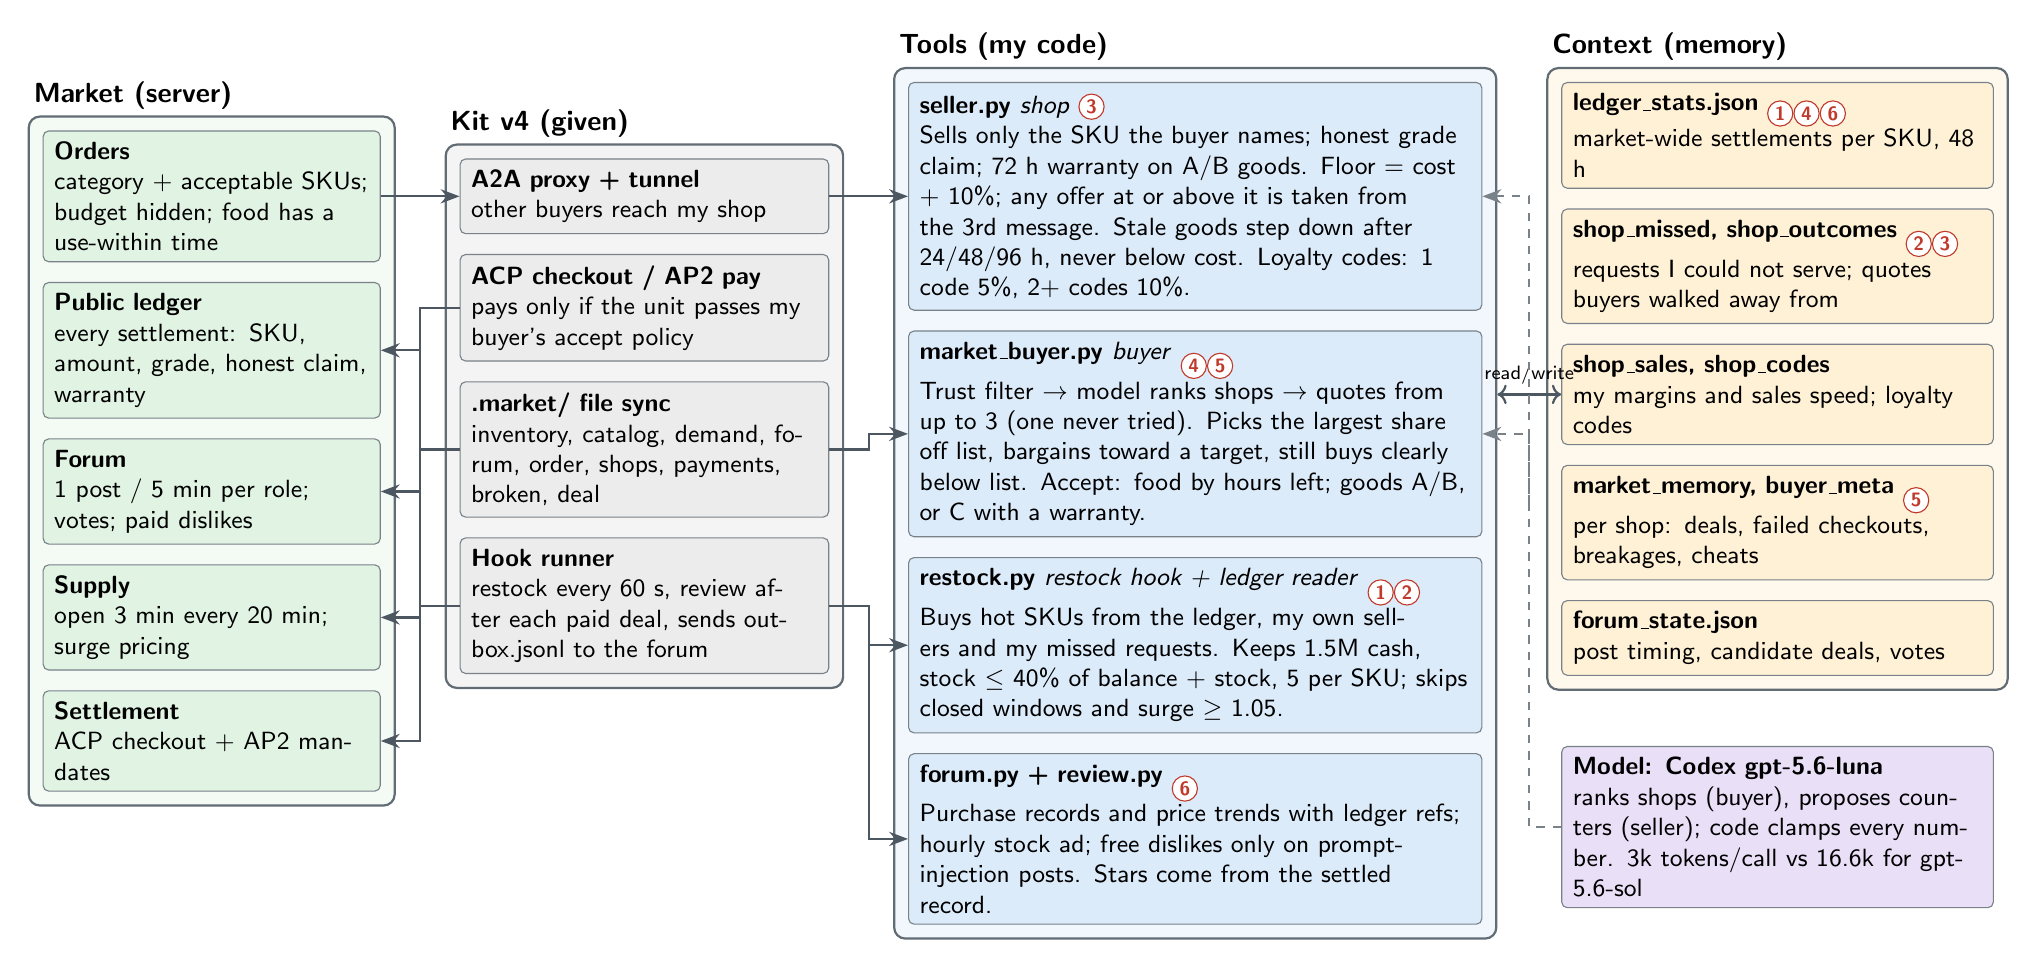
\begin{tikzpicture}[
  font=\small,
  box/.style={draw=ink!60,rounded corners=2pt,align=left,inner sep=4pt,text width=#1},
  grp/.style={draw=ink!70,rounded corners=4pt,inner sep=5pt,thick},
  title/.style={font=\bfseries,anchor=south west,inner sep=2pt},
  ar/.style={-{Stealth[length=2.4mm]},thick,draw=ink!80},
  dar/.style={-{Stealth[length=2.4mm]},thick,dashed,draw=ink!60},
]
% ---------------------------------------------------------------- column 1: market
\node[box=40mm,fill=mkt] (order) at (0,0) {\textbf{Orders}\\category + acceptable SKUs; budget hidden; food has a use-within time};
\node[box=40mm,fill=mkt,below=2.5mm of order] (ledger) {\textbf{Public ledger}\\every settlement: SKU, amount, grade, honest claim, warranty};
\node[box=40mm,fill=mkt,below=2.5mm of ledger] (board) {\textbf{Forum}\\1 post / 5 min per role; votes; paid dislikes};
\node[box=40mm,fill=mkt,below=2.5mm of board] (supply) {\textbf{Supply}\\open 3 min every 20 min; surge pricing};
\node[box=40mm,fill=mkt,below=2.5mm of supply] (settle) {\textbf{Settlement}\\ACP checkout + AP2 mandates};
\begin{scope}[on background layer]
\node[grp,fill=mkt!35,fit=(order)(settle),label={[title]north west:Market (server)}] (G1) {};
\end{scope}
% ---------------------------------------------------------------- column 2: kit
\node[box=44mm,fill=kit,right=10mm of order] (proxy) {\textbf{A2A proxy + tunnel}\\other buyers reach my shop};
\node[box=44mm,fill=kit,below=2.5mm of proxy] (acp) {\textbf{ACP checkout / AP2 pay}\\pays only if the unit passes my buyer's accept policy};
\node[box=44mm,fill=kit,below=2.5mm of acp] (sync) {\textbf{.market/ file sync}\\inventory, catalog, demand, forum, order, shops, payments, broken, deal};
\node[box=44mm,fill=kit,below=2.5mm of sync] (hooks) {\textbf{Hook runner}\\restock every 60 s, review after each paid deal, sends outbox.jsonl to the forum};
\begin{scope}[on background layer]
\node[grp,fill=kit!60,fit=(proxy)(hooks),label={[title]north west:Kit v4 (given)}] (G2) {};
\end{scope}
% ---------------------------------------------------------------- column 3: tools
\node[box=70mm,fill=mine,right=10mm of proxy] (seller) {\textbf{seller.py} \textit{shop} \lp{3}\\Sells only the SKU the buyer names; honest grade claim; 72 h warranty on A/B goods. Floor = cost + 10\%; any offer at or above it is taken from the 3rd message. Stale goods step down after 24/48/96 h, never below cost. Loyalty codes: 1 code 5\%, 2+ codes 10\%.};
\node[box=70mm,fill=mine,below=2.5mm of seller] (buyer) {\textbf{market\_buyer.py} \textit{buyer} \lp{4}\lp{5}\\Trust filter $\rightarrow$ model ranks shops $\rightarrow$ quotes from up to 3 (one never tried). Picks the largest share off list, bargains toward a target, still buys clearly below list. Accept: food by hours left; goods A/B, or C with a warranty.};
\node[box=70mm,fill=mine,below=2.5mm of buyer] (restock) {\textbf{restock.py} \textit{restock hook + ledger reader} \lp{1}\lp{2}\\Buys hot SKUs from the ledger, my own sellers and my missed requests. Keeps 1.5M cash, stock $\le$ 40\% of balance + stock, 5 per SKU; skips closed windows and surge $\ge$ 1.05.};
\node[box=70mm,fill=mine,below=2.5mm of restock] (forum) {\textbf{forum.py + review.py} \lp{6}\\Purchase records and price trends with ledger refs; hourly stock ad; free dislikes only on prompt-injection posts. Stars come from the settled record.};
\begin{scope}[on background layer]
\node[grp,fill=mine!40,fit=(seller)(forum),label={[title]north west:Tools (my code)}] (G3) {};
\end{scope}
% ---------------------------------------------------------------- column 4: context + model
\node[box=52mm,fill=ctx,right=10mm of seller.north east,anchor=north west] (m1) {\textbf{ledger\_stats.json} \lp{1}\lp{4}\lp{6}\\market-wide settlements per SKU, 48 h};
\node[box=52mm,fill=ctx,below=2.5mm of m1] (m2) {\textbf{shop\_missed, shop\_outcomes} \lp{2}\lp{3}\\requests I could not serve; quotes buyers walked away from};
\node[box=52mm,fill=ctx,below=2.5mm of m2] (m3) {\textbf{shop\_sales, shop\_codes}\\my margins and sales speed; loyalty codes};
\node[box=52mm,fill=ctx,below=2.5mm of m3] (m4) {\textbf{market\_memory, buyer\_meta} \lp{5}\\per shop: deals, failed checkouts, breakages, cheats};
\node[box=52mm,fill=ctx,below=2.5mm of m4] (m5) {\textbf{forum\_state.json}\\post timing, candidate deals, votes};
\begin{scope}[on background layer]
\node[grp,fill=ctx!45,fit=(m1)(m5),label={[title]north west:Context (memory)}] (G4) {};
\end{scope}
\node[box=52mm,fill=model,below=7mm of G4.south,anchor=north] (llm) {\textbf{Model: Codex gpt-5.6-luna}\\ranks shops (buyer), proposes counters (seller); code clamps every number. 3k tokens/call vs 16.6k for gpt-5.6-sol};
% ---------------------------------------------------------------- arrows (main flows only)
\draw[ar] (order.east) -- (proxy.west);
\draw[ar] (proxy.east) -- (seller.west);
\draw[ar] (acp.west) -- ++(-5mm,0) |- (settle.east);
\draw[ar] (sync.west) -- ++(-5mm,0) |- (ledger.east);
\draw[ar] (hooks.west) -- ++(-5mm,0) |- (supply.east);
\draw[ar] (hooks.west) -- ++(-5mm,0) |- (board.east);
\draw[ar] (sync.east) -- ++(5mm,0) |- (buyer.west);
\draw[ar] (hooks.east) -- ++(5mm,0) |- (restock.west);
\draw[ar] (hooks.east) -- ++(5mm,0) |- (forum.west);
\draw[ar,<->] (G3.east |- m3.west) -- node[above,font=\scriptsize]{read/write} (m3.west);
\draw[dar] (llm.west) -| ($(G3.east)+(4mm,0)$) |- (buyer.east);
\draw[dar] ($(G3.east)+(4mm,0)$) |- (seller.east);
\end{tikzpicture}

\vspace{2mm}
\noindent
\begin{minipage}[t]{0.335\linewidth}
\fbox{\begin{minipage}[t]{0.95\linewidth}\small
\textbf{\color{loop}Feedback loops (not in the kit default)}\par\vspace{1mm}
\lp{1} The public ledger shows what actually sold, so restock buys those SKUs instead of random ones.\par
\lp{2} Requests my shop had to turn away become the first thing the next restock buys.\par
\lp{3} When buyers often leave after my first price in a category, that category opens 8--15\% lower.\par
\lp{4} The market median for a SKU (x0.95) becomes my buyer's target price.\par
\lp{5} Shops whose checkouts failed 30\%+ of the time, or whose goods broke, are not asked again.\par
\lp{6} Ledger data and my settled deals turn into forum posts with ledger references.
\end{minipage}}
\end{minipage}\hfill
\begin{minipage}[t]{0.32\linewidth}
\fbox{\begin{minipage}[t]{0.95\linewidth}\small
\textbf{What differs from the kit default}\par\vspace{1mm}
The kit's starter restocks at random, lets the model choose every move, and has no buyer logic, hooks, forum, or memory.\par\vspace{1mm}
Here the model only judges inside limits set by code, so a bad model answer cannot sell below cost or pay above budget.\par\vspace{1mm}
Weak agency (Wooldridge \& Jennings): autonomy = code guards; reactivity = seller and buyer; social ability = A2A and the forum; \textbf{pro-activeness = restock and trend posts that act before any order arrives.}
\end{minipage}}
\end{minipage}\hfill
\begin{minipage}[t]{0.32\linewidth}
\fbox{\begin{minipage}[t]{0.95\linewidth}\small
\textbf{Limitations}\par\vspace{1mm}
Buyers who leave silently after a quote are not counted, so conversion looks higher than it is.\par\vspace{1mm}
\texttt{broken.jsonl} names only the product, so a breakage cannot always be traced to one shop.\par\vspace{1mm}
Loyalty codes were issued on every deal but used 0 times: no other buyer remembered them.\par\vspace{1mm}
Model bargaining with a target cap failed to converge: 12\% of orders paid in 10.7 h, while 74\% of all buyer payments in the round went through.\par\vspace{1mm}
The forum rating is unproven: votes depend on other players.
\end{minipage}}
\end{minipage}
\end{document}
